\documentclass[a4paper,12pt,fleqn]{article}
\usepackage[T1]{fontenc}
\usepackage{ucs}
\usepackage[utf8x]{inputenc}
\usepackage{ngerman}
\usepackage[ngerman]{babel}
\usepackage{lastpage}
\usepackage[pdftex]{color,graphicx}
\usepackage{listings}
\usepackage{pdflscape}
\usepackage{longtable}
\usepackage[inner=2cm,outer=2cm,top=1cm,bottom=1.5cm,includeheadfoot]{geometry}
\usepackage{fancyhdr}
\usepackage{url}
\usepackage{draftwatermark}
\usepackage{booktabs}
\usepackage{blindtext} 
\usepackage{framed} 
\usepackage{xcolor} 
\colorlet{shadecolor}{black} 

\usepackage{enumitem}

\SetWatermarkText{Vertraulich}
\SetWatermarkScale{4}
\SetWatermarkLightness{0.9}

\usepackage{pgfgantt}
\usepackage{amsmath,amssymb,amsfonts,amstext}
\usepackage{floatflt}
\usepackage{tikz}
\usetikzlibrary[arrows,snakes,backgrounds,shapes]
\usetikzlibrary{through}
\usetikzlibrary{calc}
\usepackage{caption}
\usepackage{subcaption}

% highlighting
\usepackage{xcolor,soul}

%---- PageLayout
\pagestyle{fancy}

\setlength{\headsep}{10mm}

\usepackage{eso-pic}

%----------------------------------------------------------------------------
% HEADER --------------------------------------------------------------------
%----------------------------------------------------------------------------
\fancyhead[R]{
  
\includegraphics[width=100pt,keepaspectratio]{img/amedo2012.png}
}

\fancyhead[C]{ Wochenbericht KW 24 }

\fancyhead[L]{
  \begin{tabular}[b]{l}
  Christoph Gnip\\
  Projekt: PRPS-Evolution
  \end{tabular}
}

%Linie oben
\renewcommand{\headrulewidth}{0.5pt}
%----------------------------------------------------------------------------


%----------------------------------------------------------------------------
%----------------------------------------------------------------------------
%----------------------------------------------------------------------------
\fancyfoot[L]{Stand: \today}
\fancyfoot[C]{ EXTERN }
\fancyfoot[R]{\thepage{} von \pageref{LastPage}}

% Linie unten
\renewcommand{\footrulewidth}{0.5pt}
%----------------------------------------------------------------------------

% Import Macros  ------------------------------------------------------------
\newcommand\nn{\newline\newline}

%----------------------------------------------------------------------------
% Start the Document --------------------------------------------------------
%----------------------------------------------------------------------------
\begin{document}

\setlength{\headheight}{36pt}

\begin{titlepage}


%- the Title page --------------------------------------------------------
\begin{center}
%\vspace*{2.5cm}
{\Huge \textbf{Wochenbericht KW 22}\par}
\vspace{1cm}
{\Huge 3.6. - 9.6.2013\par}
\vspace{1cm}
{\Huge Projektwoche: 7\par}

\vspace{2cm}

\large{Erstellt durch}\\
\Large{\textbf{Christoph Gnip}}


\vspace{4cm}

\Large{\textbf{Extern}}

\vfill

{\normalsize Fachbereich Elektrotechnik und angewandte Naturwissenschaften\\
Westfälische Hochschule\\[2ex]Juni 2013}


\end{center}
\newpage

\end{titlepage}

%- Section 1 ----------------------------------------------------------------
\section[Allgemeines]{Allgemeines}
%
%- Section 2 ----------------------------------------------------------------
\section[Fortschritt]{Projektfortschritt}
%
In dieser Woche wurden die Algorithmen verifiziert. Die Permutationen und die Koeffizienten werden korrekt berechnet. Es wurde mit der Umsetzung der Excel Referenzimplementation in ein C++ Modul begonnen.
%
%- Section 2.1 --------------------------------------------------------------
\subsection{Umsetzung Algorithmus}
In dieser Woche wurde begonnen den Algorithmus in ein C++ Modul zu portieren. Um den Compilevorgang zu automatisieren und Plattformunabhängigkeit zu gewährleisten, wurde ein CMake-Skript erstellt. Das Skript steuert erstellt das eigentliche Makefile, das im Anschluss ausgeführt werden kann. Im CMakefile kann auch eine Referenz auf deinen Cross-Compiler angegeben werden, sodass gegen die Architektur eines beliebigen Zielsystems compiliert werden kann. Die Umsetzung konnte in dieser Woche nicht abgeschlossen werden.
%
%- Section 2.2 --------------------------------------------------------------
\subsection{Erweiterte Betrachtung der Kondition}
In der letzten Woche wurde das Modell umgestellt, das führte im Wesentlichen zu eine Erweiterung der Matrix. Aus dieser Form ergeben sich einige Vorteile für Implementation und Verifikation, jedoch sind nun auch die Messwerte Teil der Matrix. Das macht die Konditionszahl variabel und Abhängig von den gemessenen Messwerten.\\
Im Folgenden wurde Untersucht inwieweit, die Zerlegung in Blockmatrizen und die Untersuchung der Kondition dieser, eine Abschätzung der vollständigen Konditionszahl im allgemeinen darstellt. 
\begin{equation}
\mathbf{A}=\bigg( \mathbf{Z}\quad \mathbf{P}\quad \mathbf{V}\bigg)
\end{equation}
Dabei ist:
\begin{equation}
\mathbf{Z} \in \mathbb{R}^{3x3} \quad \mathbf{P} \in \mathbb{R}^{3x3} \quad \mathbf{V}\in \mathbb{R}^{4x3}
\end{equation}
Die Matrizen $\mathbf{Z}$ und $\mathbf{P}$ sind statisch. Hingegen enthält die Matrix $\mathbf{V}$ die gemessenen Phasenwerte $\Theta_k$ der Antennen für diese Konfiguration. \\
%
Zur Zeit wird nach Literatur gesucht, die diese Überlegungen stützen.\\
%
Die Abbildung~\ref{fig:CondNumberAnalyze} zeigt die bereits angestellte Untersuchung zu dieser Überlegung. Abbildung~\ref{fig:AnalyzeOf3x3} stellt die Konditionszahl der rein geometrischen $3\times3$-Matrix dar. In der Abbildung~\ref{fig:AnalyzeOf10x3} sehen wir die Kondition der erweiterten Matrix. Neben der geometrischen sind auch die beiden anderen Blockmatrizen in diese Konditionsbetrachtung eingeflossen. Als zusätzliche Angabe wird ist sind die Skalierungsfaktoren angegeben. Legt man beide Grafiken übereinander erkennt man:
\begin{enumerate}
\item Geometrisch gut konditionierte Konfigurationen (linke Grafik), bleiben im erweiterten Modell (rechte Grafik) weiterhin gut konditioniert.
\item Die Konditionszahl der \textit{schlechteste} ist wesentlich kleiner (ca. Faktor $10$) als im rein geometrischen Modell
\end{enumerate} 
%
\begin{figure}
         \centering
         \begin{subfigure}[h]{0.5\textwidth}
                 \centering
                 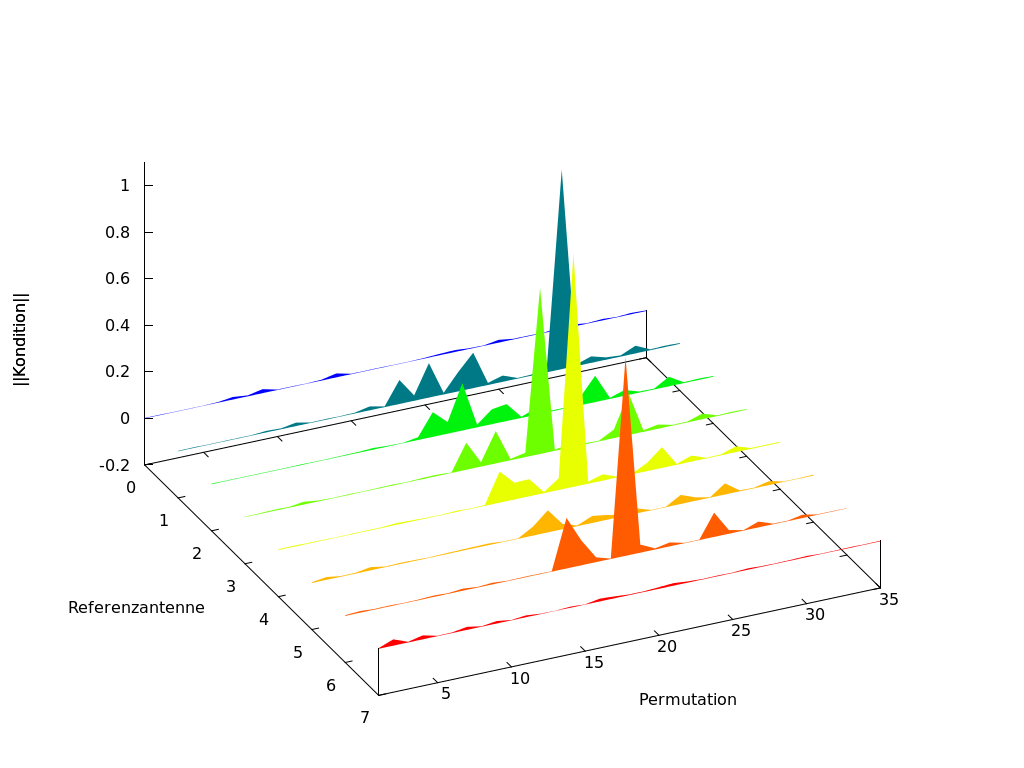
\includegraphics[width=\textwidth]{common/img/fenceModell3x3.png}
                 \caption{Konditionszahl der rein geometrischen $3\times3$ Matrix normiert auf den größten vorkommenden Wert ($=2149,16                 $)}
                 \label{fig:AnalyzeOf3x3}
         \end{subfigure}
%         
         \begin{subfigure}[h]{0.5\textwidth}
                 \centering
                 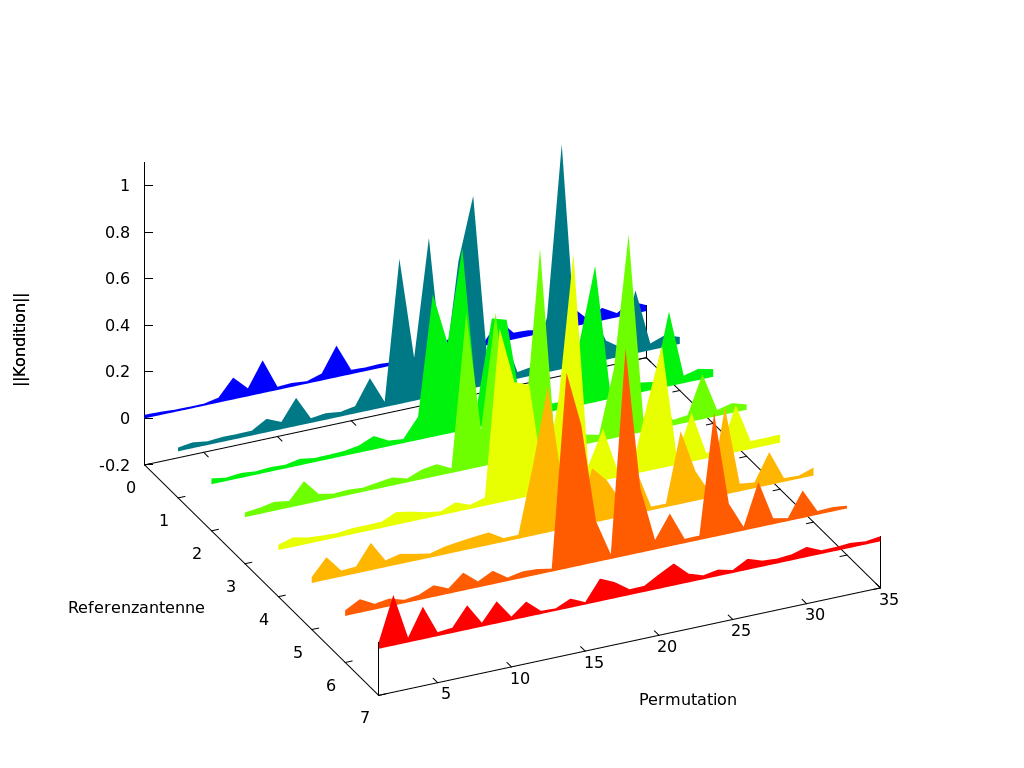
\includegraphics[width=\textwidth]{common/img/fenceModell9x3.png}
                 \caption{Konditionszahl der $10\times3$ Matrix normiert auf den größten vorkommenden Wert ($=257,13$); In dieser Konfiguration sind die Konstanten ($a_1$ \& $a_2$) sowie die variablen, gemessenen Phasen $\Theta_k$ enthalten}
                 \label{fig:AnalyzeOf10x3}
         \end{subfigure}
%
         \caption{Analyse der Konditionszahlen aller möglichen Matrizen für den Messaufbau; Die Konditionszahl ist für jede mögliche Permutation an Messantennen für eine Referenzantenne angegeben}\label{fig:CondNumberAnalyze}
\end{figure}
%
Die Grafik zeigt weiterhin, dass es für jede Referenzantenne aus der Geometrie alleine gute Konfigurationen existieren. Aus diesen Erkenntnissen kann in späteren Aufbauten, die Position der Antennen optimiert werden. Ziel der Optimierung wäre es, die Anzahl der Antennenpermutationen mit kleiner Konditionszahl zu maximieren.
%
%- Section 2.3 --------------------------------------------------------------
\subsection{Anwendung der Kondition}
Weitere Anwendung, die sich aus der Konditionszahl der Matrix ableiten, ist denkbar. Für die FPGA-Software ist, parallel zu diesem Projekt, eine intelligente Umschaltung der Antennen in der Planung. Die Kondition der geometrische Matrix verändert sich nach dem Kalibrieren nicht mehr. Dadurch und durch die oben beschriebenen Überlegungen kann statisch eine Abschätzung für die Konditionszahl, von zwei der drei Blockmatrizen, im Vorfeld erstellt werden. Die Konditionszahl dient zum Steuern der Umschaltung. Ordner man die möglichen Konfiguration anhand ihrer Konditionszahl (niedrigste zuerst) in einer statischen Liste an so kann im FPGA eine einfache, schlaue Umschaltung implementiert werden. Diese würde immer dafür sorgen, dass Messdaten von einer Konfiguration bevorzugt werden, die eine niedrige Konditionszahl hat und somit relativ sicher zu einer guten Lösung führen.
%
\subsection{Besprechung am Mittwoch}
Am Mittwoch fand eine weitere Besprechung mit Fr. Susanne Winter statt. Mit ihr wurden einige Fragen zur Messdatenaufnahme sowie zur Gestalt der Messdaten erörtert. Ein weiteres Gespräch wird voraussichtlich in der nächsten Woche stattfinden. Geplant ist bei diesem Treffen Implementationsdetails für die Shark-Library zu besprechen, da Fr. Winter Anwendungserfahrung mit dieser Library hat.
%
%- Section 3 -----------------------------------------------------------------
\section{Probleme}
\label{Problems}
Es liegen immer noch keine weiteren Messdaten vor. Die Entwicklung des FPGA-Systems wird parallel vorangetrieben.
%
%- Appendix ------------------------------------------------------------------
%
%
%
\begin{appendix}

%----------------------------------------------------------------------------
%----------------------------------------------------------------------------
%----------------------------------------------------------------------------
\newpage

\begin{center}
	\huge{Anhänge}
\end{center}

\normalsize

%----------------------------------------------------------------------------
%----------------------------------------------------------------------------
%----------------------------------------------------------------------------
\newpage
\begin{landscape}
	\section{Projektlaufplan KW 24}
	\label{sec:projectplan}
	\scalebox{.75}{
		\begin{ganttchart}[vgrid={draw=none,*1{gray, dashed}},
				hgrid=true,
				today=14,
				title height=1,
				y unit title=0.6cm,
				y unit chart=0.8cm,
				group right shift=0,
				group top shift=.3,
				group height=.3,
				milestone width=.8,
				group peaks={}{}{.2},
				incomplete/.style={fill=black!15}, %
				bar/.style={fill=white}, %
				today label={Heute},
				today rule/.style={dashed, thick}]{44}


\gantttitle{\textbf{2013}}{44} \\
\gantttitlelist{16,...,37}{2} \\
%-------------------------------------------------------------
\ganttgroup{Projekt Evaluation}{3}{14} \\
\ganttbar[progress=100, progress label font=\small\color{black!75},
	progress label anchor/.style={right=4pt}]{Installation der Umgebungen}{3}{6} \\
	
\ganttbar[progress=100, progress label font=\small\color{black!75},
	progress label anchor/.style={right=4pt},
	bar label font=\normalsize\color{black},
	name=rech]{Recherche}{3}{7} \\
	
\ganttmilestone[name=ms1]{Vorstellung der Ergebnisse}{7} \\
	
\ganttbar[progress=90, progress label font=\small\color{black!75},
	progress label anchor/.style={right=4pt},
	bar label font=\normalsize\color{black},
	name=pflichten]
	{Pflichtenheft}{5}{8} \\
	
\ganttmilestone[name=ms2]{Pflichtenheft fertig}{8} \\

\ganttbar[progress=90, progress label font=\small\color{black!75},
	progress label anchor/.style={right=4pt},
	bar label font=\normalsize\color{black},
	name=bNumVerf]
	{Einarbeitung num. Verfahren}{5}{16} \\

\ganttbar[progress=50, progress label font=\small\color{black!75},
	progress label anchor/.style={right=34pt},
	bar label font=\normalsize\color{black},
	name=bCMAES]
	{speziell CMA-ES}{7}{10} \\

\ganttmilestone[name=ms3]{Beurteilung num. Verfahren}{16} \\

\ganttlinkedbar[progress=10, progress label font=\small\color{black!75},
	progress label anchor/.style={right=34pt},
	bar label font=\normalsize\color{black}]
	{Shark Einarbeitung}{17}{18} \\

\ganttlinkedmilestone[name=ms7]{Abschluss Evaluation}{18} \\
	
%-------------------------------------------------------------
\ganttgroup{Erstellung Prototyp}{15}{26} \\
\ganttgroup{(optional)}{15}{18} \\
\ganttbar[progress=25, progress label font=\small\color{black!75},
	progress label anchor/.style={right=4pt},
	bar label font=\normalsize\color{black}]
	{(Entwurf digi. Filter)}{15}{15} \\

\ganttlinkedbar[progress=10, progress label font=\small\color{black!75},
	progress label anchor/.style={right=4pt},
	bar label font=\normalsize\color{black},
	name=bImpFPGA]
	{(Implementation FPGA)}{16}{18} \\

\ganttmilestone[name=ms4]{(Verifikation dig. Filter)}{18} \\
	
\ganttbar[progress=40, progress label font=\small\color{black!75},
	progress label anchor/.style={right=4pt},
	bar label font=\normalsize\color{black},
	name=bImplAlgo]
	{Implementation Algorithmus}{15}{26} \\

\ganttlinkedmilestone[name=ms5]{Implementation Done}{26} \\

%-------------------------------------------------------------
\ganttgroup{Verifikation}{27}{34} \\
\ganttbar[progress=10, progress label font=\small\color{black!75},
	progress label anchor/.style={right=4pt},
	bar label font=\normalsize\color{black},
	name=bVerf]
	{Durchf\"uhrung Verifikation}{27}{34} \\

\ganttlinkedmilestone[name=ms6]{Verifikation Done}{34} \\

%-------------------------------------------------------------
\ganttgroup{Projektdokumentation}{35}{42} \\

\ganttbar[progress=0, progress label font=\small\color{black!75},
	progress label anchor/.style={right=4pt},
	bar label font=\normalsize\color{black},
	name=thesis]
	{Thesis schreiben}{35}{42} \\
	
\ganttmilestone[name=msthesis,milestone label font=\color{red}, 
	milestone/.style={fill=red}]{Abgabe}{42}

%\ganttlink{ms7}{bImplAlgo}
\ganttlink{bImpFPGA}{ms4}
\ganttlink{bNumVerf}{ms3}
\ganttlink{bCMAES}{ms3}
\ganttlink{rech}{ms1}
\ganttlink{pflichten}{ms2}
\ganttlink{thesis}{msthesis}

	\end{ganttchart}
		}
\end{landscape}

%----------------------------------------------------------------------------

\end{appendix}


\newpage
%- Bibliography --------------------------------------------------------------
\bibliographystyle{ieeetr}
\bibliography{../bib/mathesis_collection1}

\end{document}